\documentclass[12pt]{article}

\usepackage[T1]{fontenc}
\usepackage[utf8]{inputenc}
\usepackage{lmodern}
\usepackage{fullpage}
\usepackage[hidelinks]{hyperref}
\usepackage{graphicx}

\title{A Neutral News Aggregator}
\author{Pranav Dahiya}
\date{1710110249}

\begin{document}

\maketitle

\section{Introduction}
\label{sec:introduction}

Today, we are in the age of information. We have access to all of human knowledge, ever created, at our fingertips, available instantly through powerful search engines. Not only that, we also have access to instant reliable communication via text, audio and video, with not just people on Earth, but also astronauts in space. This is truly a miracle. From the advent of the first general purpose computer, the ENIAC, in 1951, and the first iteration of the modern internet in 1983 with the introduction of TCP/IP, we have achieved almost global penetration of computing devices and the internet in the span of a few short decades. However, with such rapid advances, has also come rapid change. The way in which we live our lives today, in which we perform daily tasks, would have been unimaginable to person living in even the most developed economies of the world less than a century ago. Just as with everything else, the way in which we consume news and stay up to date with the rest of the world has also been transformed by the advent of modern technology.\\

The popularity of print media has been steadily declining in the past few decades, just as digital media is taking off. After all, producing content online is easier, cheaper, and more accessible to a wider audience. This has resulted in the production of so many articles every single day, that would be impossible to read by a human in an entire lifetime. Therefore, it is no wonder that more and more people are relying on news aggregators every day. According to \cite{doh-shin16}, 80\% of online news readership relies on some form of news aggregation. These news aggregators aim to simplify the untamed landscape of the modern internet by crawling the web, and finding the most important, the most relevant, and the best quality news articles, specifically curated to your personal tastes and preferences.\\

But, as with every new technology, news aggregators have both pros and cons. In an increasingly polarized world, news aggregator and social media (another popular source of news today) algorithms have come under fire for prioritizing user engagement over quality and truth. Recent studies have shown that fake news spreads faster than real news on such platforms \cite{Vosoughi18}, that these platforms reduce the diversity of news that a user sees \cite{claussens19} and result in filter bubbles \cite{berman20} that promote confirmation bias rather than facts \cite{hu19, ling20}. News aggregators such as Google News have also been shown to favor certain types of news outlets over other \cite{fischer20}. In addition, since the primary news provider is now an aggregator, rather than a known newspaper or website, readers do not pay attention to the source of the news \cite{antonis19} which provides an avenue for media outlets that do not necessarily rely on facts in their reporting to become popular.\\

Not having a news aggregator is also not an option. At the end of the day, they do accomplish their objective of increasing readership of news. As shown by \cite{calzada20}, when Spain passed legislation in 2014, forcing Google News to leave the Spanish market, readership on Spanish news websites immediately dropped by over 10\% in some cases. Therefore, there is a need for a news aggregator that is open about its algorithms, and allows users to customize how, and from where, they receive their daily news.

\section{Technology}

This section outlines the technology stack of the application and how it is built. The objective of the development process has been to prototype a news aggregator that solves the problems outlined in section \ref{sec:introduction} with a scalable architecture. The application achieves its goals by incorporating features of both modern news aggregators and traditional RSS feed readers. The news articles are compiled from feeds chosen by the user, just like in RSS readers, but clutter is reduced by organizing incoming articles into categories by clustering and ranking articles within categories for importance. The architecture of the application is as follows:
\begin{itemize}
  \item There is a web server that is constantly scraping news sources, downloading articles and adding them the database. This script also vectorizes incoming articles using doc2vec.
  \item There is an api that serves requests from clients. The http request contains feeds the user wants to see, and categories are returned. Once the user clicks on a category, articles in the category are returned. 
  \item Rendering of the article takes place at the client.
\end{itemize}
The source code for this project can be found at \href{https://www.github.com/pranav-dahiya/News}{this git repo}.

\subsection{Backend}

The webserver was containerized using docker, in order to make the application scalable and portable. The webserver, and the database run in their own containers based on the python and mysql images from docker hub. The Dockerfiles and compose files are included in the source code.\\

MySQL was used as the database of choice. The database schema can be found in figure \ref{fig:schema}.\\

\begin{figure}
  \centering
  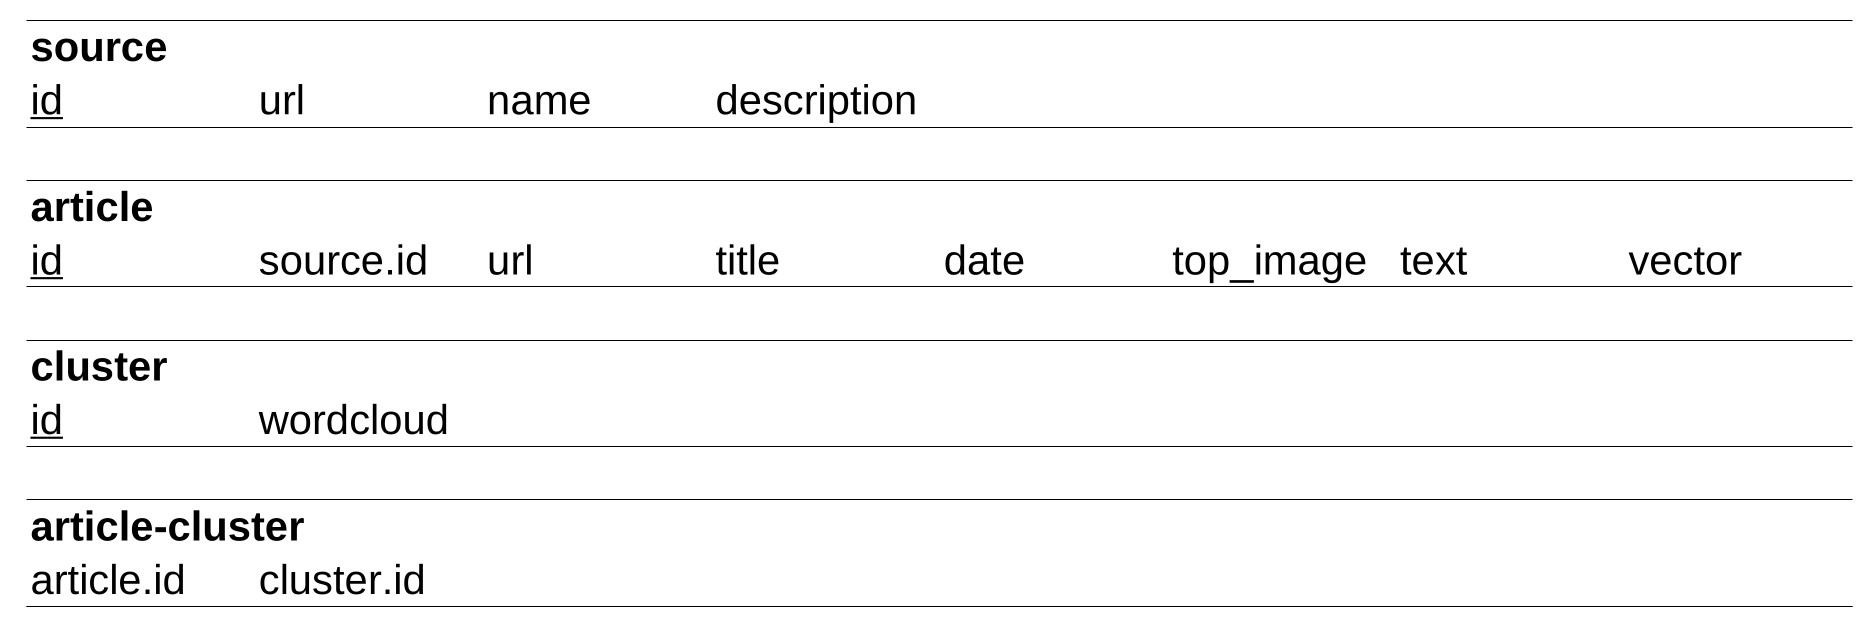
\includegraphics[width=\textwidth]{db_schema.jpg}
  \caption{Database Schema}
  \label{fig:schema}
\end{figure}

Articles were scraped from the web using the newspaper3k library in python. They were vectorized using the doc2vec model found in gensim, trained on the included Wikipedia corpus. After vectorizing, clustering was done using Latent Dirichlet Allocation (LDA) in pyspark. For more information on doc2vec and LDA, the reader is directed to \cite{le14} and \cite{blei03}. Flask was used to create the API.\\

Currently, the webserver is hosted on my own personal machine running Arch Linux with an Intel i7-8750H 6 core processor and 16GB of RAM. Despite relatively powerful specs, the system was still limited by the processing power and memory, therefore, it was not feasible to go for cloud hosting. However, since everything is running in its own container, it should be easy to move the server to any other machine, either locally or on the cloud.

\subsection{Frontend}

The frontend was created in PyGTK+ because it integrates well with the Gnome desktop environment on my machine. The requests library was used to interface with the API and webkit2 was used to render webpages of the news articles. For now, the customization of feed sources is done through dot files stored locally at the client.

\section{Novelty}

Existing solutions essentially fall in one of three categories:
\begin{itemize}
  \item \textbf{Smart News Aggregator}: Examples include InShorts and Google News. These services aim to declutter the world of digital news, but suffer from limitations highlighted in section \ref{sec:introduction}.
  \item \textbf{RSS Feed Readers}: Examples include Feedly and Palabre. These services allow users to set their news sources and update with new articles as they become available. However, they suffer from information overload. So many articles are published every day, that even with a handful of sources, the user can expect to see 100s if not 1000s of articles daily.
  \item \textbf{Reading News Directly on Media Websites}: This solution suffers from low engagement with users. Users are much less likely to go through the effort of bookmarking multiple websites or downloading multiple apps, and opening each source regularly to check for updates.
\end{itemize}

The solution presented in this project aims to mitigate the issues with existing solutions. In addition to this, the following secondary objectives of this project also set it apart from your average news aggregator:
\begin{itemize}
  \item \textbf{Free and Open Source Software}: This news reader is free and the source code is available online. Therefore, users can rest assured that they are seeing the news that they want to see, and not what some algorithm has decided after maximizing on user engagement.
  \item \textbf{Privacy}: There is no account linked to the news reading habits. All user data is locally stored, in human readable and editable format, ensuring that users' activity is not being tracked.
  \item \textbf{Customizability}: You decide what news you want to see, and when you want to see it. If the user no longer wants to subscribe to a news outlet, it can be removed, and similarly, additional news sources can be added. 
  \item \textbf{Simplicity}: The application UI is designed with simplicity in mind. The user gets news articles, a refresh button, a back button, and that's it. No more complicated RSS feed settings or pesky ads.
\end{itemize}

\section{Conclusion and Future Work}

The goals set out in the beginning of the project have been accomplished. However, there are many more features that could improve the user experience, and further increase the usability of this software as a full fledged news reader and aggregator:
\begin{itemize}
  \item While the current clustering model serves its purpose to demonstrate the functioning of this application, it is by no means perfect. A lot of work can be done in improving the underlying algorithm and making the clusters better defined and more meaningful.
  \item Since this an open and privacy focused news reader, the option for self hosting would be really helpful. Nextcloud is a popular self hosted cloud storage service that relies on free and open source software. Nextcloud integration can be baked into the application so that it can simply be installed with one click from the Nextcloud app store and run on the user's own server.
  \item More features can be brought into the GUI such as editing feed sources, customizing the number of articles that are returned in one go, searching for articles, and setting date filters.
  \item More options could be provided for the frontend such as a version in PyQt that will have better compatibility with other desktop environment in Linux, and with Windows 10, or an Android client.
\end{itemize}


\bibliography{bibliography}{}
\bibliographystyle{plain}

\end{document}
